\documentclass[conference]{IEEEtran}
\IEEEoverridecommandlockouts
% The preceding line is only needed to identify funding in the first footnote. If that is unneeded, please comment it out.
\usepackage{cite}
\usepackage{amsmath,amssymb,amsfonts}
\usepackage{graphicx}
\usepackage{textcomp}
\usepackage{xcolor}
\usepackage{fancyvrb}
\usepackage{listings}
\usepackage{hyperref}
\usepackage{times}
\usepackage{letltxmacro}

\lstset{basicstyle=\scriptsize\ttfamily,breaklines=true}

\def\BibTeX{{\rm B\kern-.05em{\sc i\kern-.025em b}\kern-.08em
    T\kern-.1667em\lower.7ex\hbox{E}\kern-.125emX}}
\begin{document}

\title{Application of BagIt-Serialized Research Object Bundles for Packaging and Re-execution of Computational Analyses}

\author{

\IEEEauthorblockN{Kyle Chard}
\IEEEauthorblockA{\small{Computation Institute} \\
University of Chicago\\
Chicago, IL \\
chard@uchicago.edu}\\

\IEEEauthorblockN{Niall Gaffney}
\IEEEauthorblockA{\small{Texas Advanced Computing Center} \\
University of Texas at Austin\\
Austin, TX \\
ngaffney@tacc.utexas.edu}\\

\IEEEauthorblockN{Matthew B. Jones}
\IEEEauthorblockA{\small{NCEAS} \\
\small{University of California at Santa Barbara}\\
Santa Barbara, CA\\
jones@nceas.ucsb.edu}\\

\IEEEauthorblockN{Kacper Kowalik}
\IEEEauthorblockA{\small{NCSA} \\
\small{University of Illinois at Urbana-Champaign}\\
Champaign, IL\\
kowalikk@illinois.edu}\\

\and

\IEEEauthorblockN{Bertram Lud\"ascher}
\IEEEauthorblockA{\small{School of Information Sciences} \\
\small{University of Illinois at Urbana-Champaign}\\
Champaign, IL \\
ludaesch@illinois.edu}\\

\IEEEauthorblockN{Jarek Nabrzyski}
\IEEEauthorblockA{\small{Center for Research Computing} \\
\small{University of Notre Dame}\\
South Bend, IN\\
jaroslaw.nabrzyski.1@nd.edu}\\

\IEEEauthorblockN{Victoria Stodden}
\IEEEauthorblockA{\small{School of Information Sciences} \\
\small{University of Illinois at Urbana-Champaign}\\
Champaign, IL \\
vcs@stodden.net} \\

\IEEEauthorblockN{Ian Taylor}
\IEEEauthorblockA{\small{Center for Research Computing} \\
\small{University of Notre Dame}\\
South Bend, IN\\
ian.j.taylor@gmail.com} \\

\and

\IEEEauthorblockN{Thomas Thelen}
\IEEEauthorblockA{\small{NCEAS} \\
\small{University of California at Santa Barbara}\\
Santa Barbara, CA\\
thelen@nceas.ucsb.edu} \\

\IEEEauthorblockN{Matthew J. Turk}
\IEEEauthorblockA{\small{School of Information Sciences} \\
\small{University of Illinois at Urbana-Champaign}\\
Champaign, IL \\
mjturk@illinois.edu} \\

\IEEEauthorblockN{Craig Willis\IEEEauthorrefmark{2}}
\IEEEauthorblockA{\small{NCSA} \\
\small{University of Illinois at Urbana-Champaign}\\
Champaign, IL\\
willis8@illinois.edu}\\ 
\IEEEauthorrefmark{2}\footnotesize{\emph{Corresponding author}}
}



\maketitle

\begin{abstract}
In this paper we describe our experience adopting the Research Object Bundle (RO-Bundle) format with BagIt 
serialization (BagIt-RO) for the design and implementation of ``tales" in the Whole Tale 
platform. A \emph{tale} is an executable research object intended for the dissemination of 
computational scientific findings that captures information needed to facilitate understanding, 
transparency, and re-execution for review and computational reproducibility at the time of publication. 
We describe the Whole Tale platform and requirements that led to our adoption of BagIt-RO, specifics 
of our implementation, and discuss migrating to the emerging Research Object Crate (RO-Crate) 
standard.
\end{abstract}

\begin{IEEEkeywords}
Reproducibility of results, Standards, Packaging, Interoperability, Software, Digital preservation
\end{IEEEkeywords}

\section{Introduction}

Whole Tale (http://wholetale.org) is a web-based, open-source platform for reproducible research 
supporting the creation, sharing, execution, and verification of ``tales" \cite{brinckman2019, chard2019}. Tales are executable research objects that capture the code, data, and environment along with narrative and workflow information needed to re-create computational results from scientific studies. A goal of the Whole Tale platform (WT) is to produce an archival package that is exportable, publishable, and can be used for verification of computational reproducibility, for example as part of the peer-review process.

Since its inception, the Whole Tale platform has been designed to bring together existing open 
science infrastructure.  Researchers can ingest existing data from various scientific archival 
repositories; launch popular analytical tools (such as Jupyter and RStudio); create and customize 
computational environments (using \texttt{repo2docker}\footnote{https://repo2docker.readthedocs.io/}); 
conduct analyses; create/upload code and data; and publish the resulting package back to an
archival repository. Tales are also downloadable and re-executable locally, including the 
ability to retrieve remotely published data.  

With the May 2019 release of version 0.7 of the platform we adopted the Research Object Bundle BagIt serialization (BagIt-RO) format \cite{soilandreyes2014}. By combining the BagIt-RO 
serialization with our repo2docker-based execution framework and the BDBag tools 
\cite{chard2016}, we were able to define and implement a standards-compliant, self-describing, 
portable, re-executable research object with the ability to retrieve remotely published data.  

In this paper we describe the Whole Tale platform and requirements that led to our adoption of the
the BagIt-RO format. The paper is organized as follows. In section \ref{scenario}, we present a 
motivating example of the  use of the Whole Tale platform followed by a brief description of the 
system architecture in section \ref{architecture}. In section \ref{requirements} we outline the 
requirements that led to our adoption of the BagIt-RO format. In section \ref{adopting} we describe
our implementation in more detail followed by a discussion and conclusions.


\section{Example scenario: Analyzing seal migration patterns} \label{scenario}
We begin with a motivating example to illustrate the end-to-end Whole Tale workflow for creating, exporting, and publishing a tale based on existing data archived using the Research Workspace\footnote{https://www.researchworkspace.com}, a DataONE member node. This example is based tutorial material described in \cite{london2018}.

\begin{quote}
A research team is preparing to publish a manuscript describing a computational model for 
estimating animal movement paths from telemetry data. The source data for their analysis, 
tracking data for juvenile seals in Alaska\cite{cameron2018}, has been published in Research 
Workspace, a DataONE network member. Using the Whole Tale platform, the researchers register the 
external dataset. They then create a new tale by launching an RStudio environment based on 
images maintained by the Rocker Project \cite{boettiger2018}. Using the interactive environment, 
they clone a Github repository, modify an R Markdown document, customize the environment by 
specifying OS and R packages via repo2docker configuration files, and execute their code to 
generate outputs. They download the package in a compressed BagIt-RO format and run locally to 
verify their tale. Finally, they enter descriptive metadata and publish the final 
package back to DataONE to archive the package and obtain a persistent identifier to include in publication. 
\end{quote}

This scenario is further illustrated in Figure \ref{workflow}.


\begin{figure*}
\centering
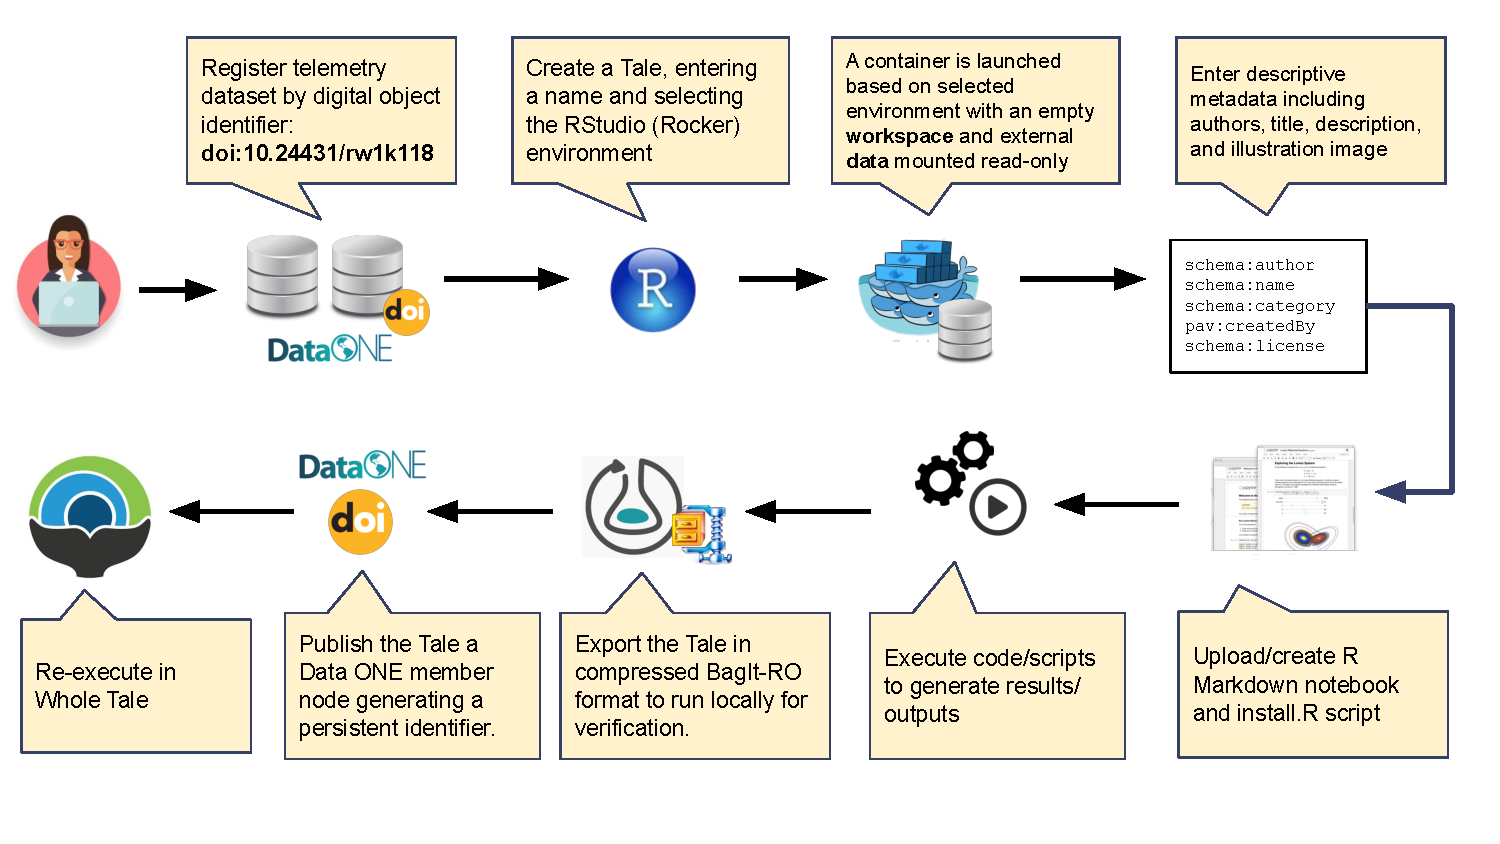
\includegraphics[scale=0.6]{images/wholetale-workflow.pdf}
\caption{Example Scenario Tale Creation and Publishing Workflow, republished from \cite{chard2019}, permission needed.}
\end{figure*}
\label{workflow}

\section{System architecture} \label{architecture}

This section provides a brief overview of the Whole Tale system architecture illustrated in Figure 
\ref{architecture}. Whole Tale 
provides a scalable platform based on the Docker Swarm container orchestration system, exposing a 
set of core services via REST APIs and Single Page Application (SPA). Key components include:

\begin{figure}
\centering
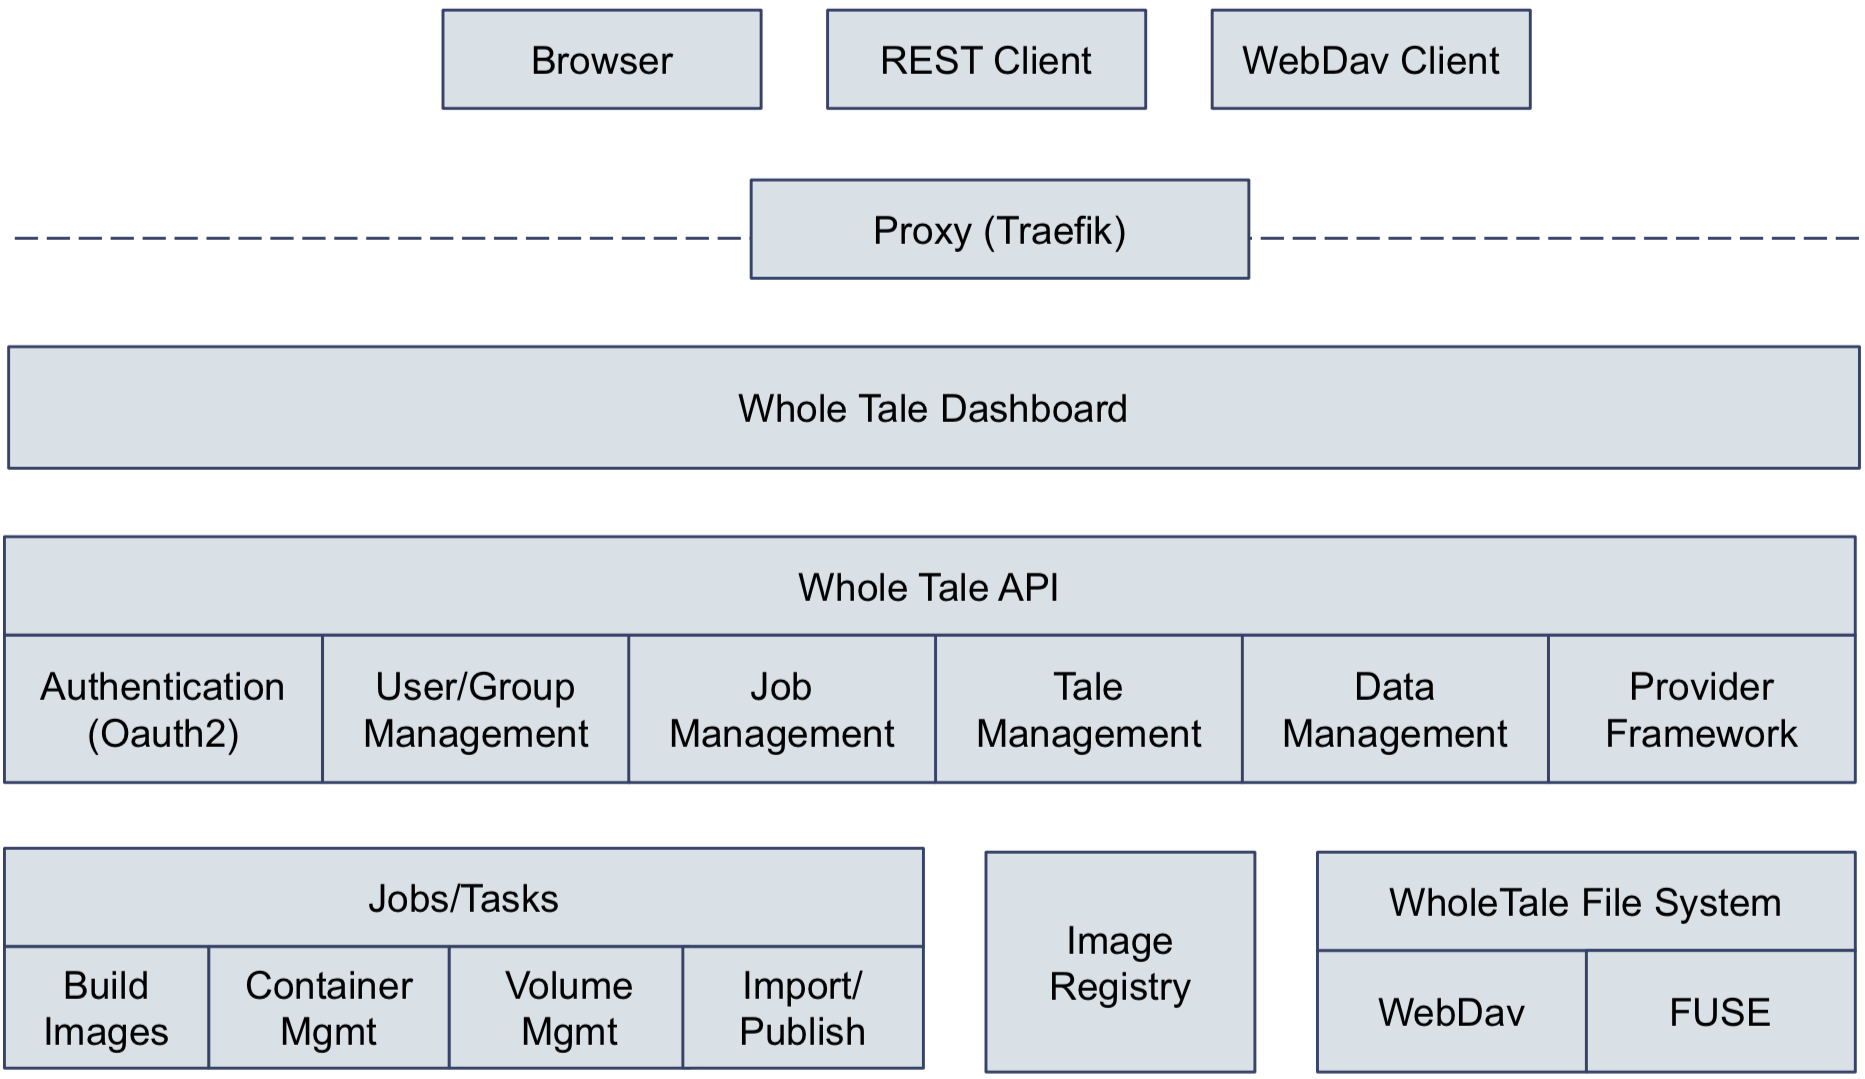
\includegraphics[scale=0.25]{images/wholetale-architecture.png}
\caption{Whole Tale system architecture}
\end{figure}
\label{architecture}

\begin{itemize}
\item{{\bf Whole Tale Dashboard}: An Ember.js single page application}
\item{{\bf Whole Tale API}: A REST API built using the Girder\footnote{https://girder.readthedocs.io} framework to expose key features including authentication, user/group management, tale lifecycle, data management, and integration with remote repositories}
\item{{\bf Whole Tale File System}: A custom filesystem based on WebDav and FUSE used to mount user and registered data into running container environments}
\item{{\bf Image registry}: A local Docker registry used to host images associated with tales}
\item{{\bf Jobs and task Management}: A task distribution and notification framework based on Girder and Celery}
\item{{\bf Data Management System (DMS)}: System for fetching, caching, and exposing externally published datasets}
\end{itemize}

Several aspects of the Whole Tale system are related to the BagIt-RO serialization format including filesystem organization, user-defined environments, metadata as well as the export and publication functions. We describe these in more detail below.

\subsubsection{Tale workspace}
Each tale has a \emph{workspace} (folder) that contains user-created code, data, workflow, documentation and narrative information. The workspace also contains repo2docker-compatible configuration files defining the tale environment, described below. This appears as the \texttt{workspace} folder mounted into the running tale environment.

\subsubsection{External data}
Optionally, each tale can include references to externally published data. The data is then registered with the Whole Tale system and managed by the DMS. Externally referenced data appears in the \texttt{data} folder, a sibling to the \texttt{workspace}.

\subsubsection{Environment customization}
Users can optionally customize the tale environment using repo2docker-compatible configuration files. Whole Tale extends repo2docker via the \texttt{repo2docker\_wholetale}\footnote{https://github.com/whole-tale/repo2docker\_wholetale} package, which adds buildpacks to support Rocker, Spark, and OpenRefine images. 

\subsubsection{Metadata}

Tales have basic descriptive metadata including creator, authors, title, description, keywords as well as information about the selected environment, licenses, and associated persistent identifiers. The tale metadata is included in the metadata directory both in the \texttt{manifest.json} and \texttt{environment.json} files.  The license is included in the BagIt payload directory, but not as part of the tale workspace.
%where is the metadata located? is it a tale object?

\subsubsection{Exporting tales}

Tales can be exported in a BagIt-RO serialized archive that contains the contents of the tale workspace (code, local data, narrative, workflow, repo2docker configuration files) as well as references to external data, tale metadata, and a script to run the tale locally. BDBag \cite{chard2016} is used to materialize ``holey" bags by downloading files specified in the \texttt{fetch.txt} file, initially via HTTP and eventually via DOI, Globus, Agave schemes.  The script to run locally is stored at the root of the exported BagIt archive.
% "tale metadata, and a script to run the tale locally." where are these stored when the tale is published?

Table 1 describes the contents of an exported tale in the BagIt-RO format. A complete example is available at \href{https://doi.org/10.5281/zenodo.2641314}{https://doi.org/10.5281/zenodo.2641314}.
% readers will wonder about the tale license and where that information is located


\begin{table}
\begin{center}
\begin{footnotesize}
\begin{tabular}{| p{3.5cm}|p{4.5cm} | } \hline
{\bf File} & {\bf Description}  \\ \hline
\texttt{bag-info.txt} & Bag metadata using the bdbag-ro-profile\footnote{https://raw.githubusercontent.com/fair-research/bdbag/master/profiles/bdbag-ro-profile.json} \\ \hline
\texttt{bagit.txt} & Bag declaration \\ \hline
\begin{minipage}{3in}
\begin{scriptsize}
\begin{verbatim}

data/
  LICENSE
  workspace/
    apt.txt
    postBuild
    requirements.txt
    wt_quickstart.ipynb
\end{verbatim}
\end{scriptsize}
\end{minipage} & Payload directory containing tale license and workspace contents including repo2docker compatible configuration files. \\ \hline
\texttt{\texttt{fetch.txt}} & Fetch file \\ \hline
\texttt{manifest-[md5, sha256].txt} & Payload manifest (checksums) \\ \hline
\begin{minipage}{3in}
\begin{scriptsize}
\begin{verbatim}

metadata/
    manifest.json
    environment.json
\end{verbatim}
\end{scriptsize}
\end{minipage} & Tag directory containing RO manifest.json and Whole Tale environment metadata  (required by repo2docker\_wholetale) \\ \hline
\texttt{tagmanifest-[md5, sha256].txt} & Tag manifest (checksums) \\ \hline
\texttt{README.md} & Tale top-level readme \\ \hline
\texttt{run-local.sh} & Tale local execution script \\ \hline
\end{tabular}
\end{footnotesize}
\label{bagitro-example}
\caption{Exported tale contents}
\end{center}
\end{table}



\section{Requirements}  \label{requirements}
The scenario described in section \ref{scenario} highlights several key requirements of the 
Whole Tale platform that led to our selection of the BagIt-RO serialization.  These requirements include:

\begin{itemize}
\item{{\bf Interoperability with archival repositories}: Since tales will be published to archival repositories including DataONE network members, we must adopt standard formats and vocabularies that facilitate interoperability. This includes the use of supported archival formats and identifiers (e.g., digital object identifiers). We also note here that some repositories do not support publishing hierarchical file structures, while many research objects contain data and code organized in folders. In the future, we plan to support publishing to Dataverse network members, the Dryad repository, and Zenodo.}
\item{{\bf Interoperability with source code management (SCM)}: For many researchers, source code repositories such as GitHub are central to their workflow in the creation of research objects. The tale format must support publishing research objects based on content in SCM repositories.}
\item{{\bf Ability to reference external data}: A central feature of the Whole Tale platform is to enable researchers to reference externally published data by persistent identifier and include references to those items in their published tales. Both in the Whole Tale web service and when executed locally, externally referenced data must be resolved prior to re-execution. Whole Tale currently supports HTTP resources as well as those published via Globus and in the future via the Agave Platform.}
\item{{\bf Ability to add metadata}: The tale format must support all metadata attributes required by DataCite and schema.org as well as attributes specific to the Whole Tale platform. In the future, we expect to also support additional metadata required by researchers in specific domains.}
\item{{\bf Ability to export and re-execute}: One feature of the system is the ability for users to export tales to a local machine. To re-run locally, we must be able to rebuild the environment (e.g., via Docker/repo2docker) and fetch remote data as needed.}
\item{{\bf Ability to store provenance information}: Future releases of Whole Tale, tales will include computational and archival provenance information.}
\item{{\bf Simplicity and understandability}: When users view the contents of an exported or published tale, they should be able to easily understand the contents and how to explore or re-execute the tale.}
\item{{\bf Verifiability}: Future releases of Whole Tale will include information to allow the automatic re-execution and verification of included results/outputs and computational workflows.}
\item{{\bf Versioning}: Since researchers iterate on their tales, share them and extend them, it is important to be able to version them over time.}
\item{{\bf Interoperability with search engines}: Google recently unveiled Dataset Search which parses and aggregates JSON-LD embedded on dataset landing pages as an effort to lower barriers for finding datasets. Choosing JSON-LD as a representation for tale metadata provides flexibility in case we decide to expose tale information for Google. It also allows for further integration with third party publishers such as Dataverse and DataONE who may expose such metadata for Google.}
\end{itemize}

\section{Adopting the BagIt-RO Model} \label{adopting}

Whole Tale uses the RDF data model to encode tale information for export and exchange. We selected  a JSON-LD representation for human readability, extensibility, compatibility with Whole Tale APIs, and potential interoperability with search engines and third party publishers. After developing an  ad-hoc internal format, we explored emerging standards in the research object space and settled on BagIt-RO for serialization. Using RO-Bundle specification and BagIt serialization in conjunction with the BDBag tools met many of our initial requirements. Additional tale metadata attributes which were not included in the BagIt-RO model could be added using vocabularies such as schema.org. Throughout this section, we use the \texttt{manifest.json} from the above example, with a complete listing included in Appendix A.

\subsection{Filesystem Artifacts}
One strong point of RO-Bundle is that it treats file system artifacts as aggregates of the 
manifest. Doing so satisfies our requirement of being able to track where files belong, enabling 
us to both export and re-import tales even in the case where we must publish a hierarchical 
structure to a repository that can only represent a flat structure. In the case of Whole Tale, 
artifacts include data that were retrieved from external repositories as well as files that the user created or uploaded into the tale workspace. The tale workspace contents are included in the payload "data/workspace" directory and the external data are fetched into the payload "data/data" directory, mirroring filesystem organization on the web-based platform.

\begin{lstlisting}
  "aggregates": [
    {
      "uri": "../data/workspace/wt_quickstart.ipynb"
    },
    {
      "uri": "../data/workspace/apt.txt"
    }
  ]
\end{lstlisting}

Workspace artifacts are easily described with a single URI entry. Some files, such as the 
system generated README.md, are tagged with additional metadata as shown below. In this case the 
additional metadata specifies the ``type" of the file as a ``HowTo".

\begin{lstlisting}
  {
    "@type": "HowTo",
    "uri": "../README.md"
  }
\end{lstlisting}

\subsection{External data}

Whole Tale supports two types of external data: data that reside in a repository identified by persistent identifier (e.g., DOI) and data that exists at a generic HTTP address. In addition to 
including information about external data in the \texttt{manifest.json}, the URL for each remote file, regardless of type, is included in the \texttt{fetch.txt} for retrieval using BDBag tools.

{\bf Generic HTTP Data}:
For data that does not belong to a remote repository, a simple bundle is created in the aggregation section. The URI points to the HTTP address where the file may be retrieved and the bundle object holds the filesystem relevant information. The combination of information allows us to retrieve the file and place it in the correct folder (i.e., data/data).

{\bf Repository Data}: 
For datasets that have been published to research repositories, additional metadata can be ingested when files are registered with the system. The individual files are described with a single bundle object, and linked to an additional structure that describes the dataset in more detail.

The following snippet describes a remote dataset that resides in DataONE and the aggregation recording the relationship between a file in that dataset and its ultimate location after 
retrieval in the payload "data" directory:


\begin{lstlisting}
 "dataset": [
   "@type": "Dataset",
   "identifier": "doi:10.5065/D6862DM8",
   "name": "Humans and Hydrology at High Latitudes...",
   "@id": "doi:10.5065/D6862DM8"
  ],
  "aggregates": [
    {
      "size": 1558016,
      "schema:isPartOf": "doi:10.5065/D6862DM8",
      "uri": "https://cn.dataone.org/cn/v2/resolve/urn:...",
      "bundledAs": {
          "filename": "usco2000.xls",
          "folder": "../data/data/"
      }
    }
]
\end{lstlisting}

\subsection{Describing the Computing Environment}
Whole Tale uses a customized version of the Binder repo2docker package. In addition to including configuration files in the workspace, Whole Tale exports information about the environment including runtime information in the tale. One shortcoming of the BagIt-RO model is that there is not a well-defined place for this metadata. To address this need, we define an additional tag file, \texttt{environment.json}, which encodes sufficient information about the environment  so that it can be re-created. The metadata contained in this file is represented as JSON and is not described using standard vocabularies. 

\subsection{Describing Additional Attributes}
A number of properties that describe additional tale attributes (e.g., authors, keywords, description, license) are defined at the manifest root. Schema.org's vocabulary sufficed for describing these general metadata fields.

Attributing authorship to a tale is a requirement for tracking researcher contributions and is also used during metadata generation with publishers. The Provenance, Authoring, and Versioning (PAV) vocabulary is used instead of schema because it is already included in by RO-Bundle: 

\begin{lstlisting}
   {
      "@id": "https://orcid.org/0000-0002-7523-5539",
      "@type": "schema:Person",
      "schema:familyName": "DeBruine",
      "schema:givenName": "Lisa"
    }
\end{lstlisting}
		
		
\subsection{Provenance Tracking}

A planned feature of Whole Tale is the ability to track executions and steps in researchers' workflows, which we call computational provenance. The BagIt-RO model includes the ability to provide provenance information through the inclusion of the \texttt{provenance.json} file. However, this is intended to capture more archival provenance information and it is unclear whether computational provenance should be included here. Whole Tale plans to use the Prov-ONE ontology\footnote{https://purl.dataone.org/provone-v1-dev}, an extension to W3C PROV\footnote{https://www.w3.org/TR/prov-overview/}.

The URI of each file in the manifest can be referenced inside the \texttt{provenance.json} file, enabling rich linkings of information. This information can also be transcribed to publisher-specific formats, provided that they support PROV. Figure \ref{prov-fig} illustrates how provenance information is rendered in DataONE.

\begin{figure}
\centering
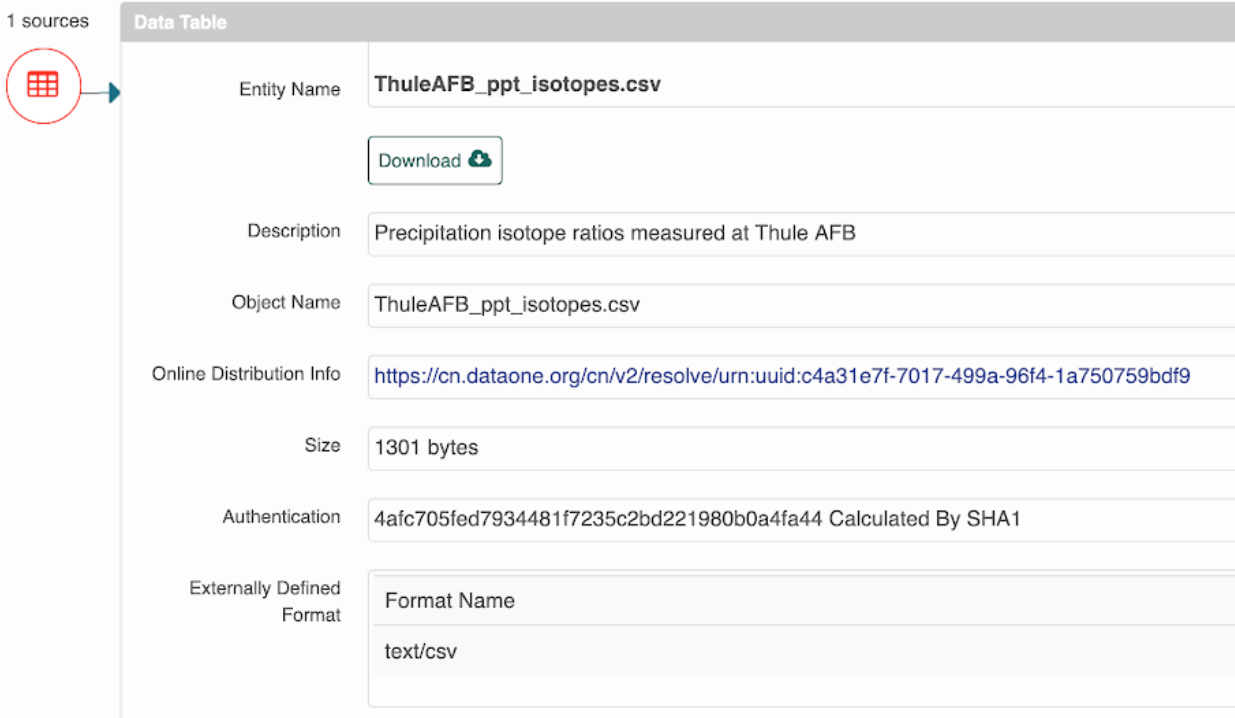
\includegraphics[scale=0.4]{images/dataone-prov.png}
\caption{Provenance rendering of a file in DataONE}
\label{prov-fig}
\end{figure}


\section{Discussion} \label{discussion}

In this section, we highlight and discuss several issues related to our implementation of BagIt-RO that we hope will be of interest to workshop participants and possible input into current work on the RO-Crate specification. We discuss the importance of re-executability; the ability to reference and retrieve external data; the relationship between tales and source control repositories; and our ongoing work on computational provenance and verification workflows.

\subsection{Executable research objects}
Tales are executable research objects. By this we mean that the research object itself may be built and re-executed for exploration, re-use, reproducibility, and verification. This is not a unique capability as many systems have recently been developed to support the creation of similar artifacts (for example Binder, CodeOcean). Executable research objects contain not only data, code, and documentation, but also information about the computational environment. This executability leads to additional capabilities, such as generation and comparison of computational provenance or methods of automated verification.

\subsection{External data}
In the Whole Tale platform, users are presented with a fixed filesystem hierarchy that includes  ``workspace'' and ``data'' directories. The workspace directory contains code, local data, and additional files (e.g., documentation) and the sibling "data" directory contains externally referenced data files (read-only).

In our v0.7 release, the BagIt payload directory of an exported tale similarly contains ``workspace'' and ``data'' directories. The \texttt{manifest.json} contains information about remotely registered datasets that is also included in the BagIt \texttt{fetch.txt}. When BDBag tools are used to fetch remote datasets, they are downloaded to the payload/data directory, matching the online filesystem organization and system capabilities. The concept of the \texttt{fetch.txt}, while primitive, is surprisingly effective when used with BDBag. We also foresee taking advantage of other BDBag capabilities, such as transferring Globus data or using DOI resolution. However, there is redundancy in tracking external information in both in the BagIt \texttt{fetch.txt} and the RO manifest.json. 

\subsection{Relationship to SCM}
Many researchers use source control repositories (e.g., GitHub) to organize and collaborate on research projects. Repositories can be released and published via external tools such as Zenodo or Whole Tale. In the Whole Tale platform, the ``workspace'' directory can be mapped to a version controlled repository. This raises the question of whether or not the workspace (or repository) should contain everything, including information currently stored in the \texttt{manifest.json} or \texttt{environment.json}. This information is essential to the understandability and re-executability of the tale, but is currently modeled as external to the primary tale contents (as is common with descriptive metadata). During the local execution process, for technical reasons we bind mount files from the ``metadata'' directory into the workspace to support building the tale 
image. In future releases, we are considering exposing the manifest information along with computational provenance information (below) as part of the workspace instead of external to it. This means that even simple metadata would be in the workspace and easily added to version control.

\subsection{Reproducibility and computational provenance information}
Computational provenance refers to methods of capturing provenance (``the source or origin of an object") for computational tasks \cite{freire2008} and is a subset of the larger notion of reproducibility of data- and computationally-enabled results \cite{stodden2013a, stodden2014a, stodden2014b, stodden2015, stodden2016}. We are beginning to explore methods of capturing and storing computational provenance information to enable reproducibility on computational findings in tales. In the RO-Bundle specification, provenance information is defined as ``describing creators, dates, and sources'' and is more concerned with the provenance of the research object itself, which we term archival provenance. Computational provenance information is internal to the tale and could be generated by the user or the Whole Tale system directly. We view computational provenance information as a key component of transparency for evaluation and verification of tales and part of enabling reproducibility.

\subsection{Supporting reproducibility via verification workflows}
Research communities and journals are increasingly adopting artifact review processes that include re-execution of computational analysis in support of reproducibility \cite{stodden2013b}. Examples include the workflow implemented by the Odum Institute for the American Journal for Political Science \cite{christian2018}, the Journal of the American Statistical Association\footnote{https://magazine.amstat.org/blog/2016/07/01/jasa-reproducible16/}, Biostatistics \cite{donoho2010}, and the ACM Transactions on Mathematical Software (TOMS) Replicated Computational Results\footnote{http://toms.acm.org/replicated-computational-results.cfm} program. We see tales and related research objects being used to simplify and possibly automate aspects of the verification process. Having a standard format for the exchange of research objects that fits into these enhanced curatorial and verification workflows may significantly reduce the burden on research communities.


\subsection{BagIt Understandability}

One drawback of the BagIt serialization is that the BagIt configuration is foregrounded and 
difficult to understand for the average researcher/user while the ``payload" directory is less 
apparent and confusingly named ``data". Although out of scope for the RO discussion, we are 
supportive of the idea of a ``.bagit" directory that contains the relevant configuration 
information and is largely hidden from the average user.


\subsection{Migrating to RO-Crate}
Since our adoption of the BagIt-RO model, the community has moved forward on the Research Object 
Crate (RO-Crate) specification\footnote{https://researchobject.github.io/ro-crate/}. In this section, we report the results of a preliminary analysis 
of changes needed to migrate to the new format. Doing so will require versioning the tale export 
format and we are unlikely to make changes until the community settles on a near-final version of the 
specification.

RO-Crate 0.2-DRAFT introduces the following changes from the RO-Bundle 1.0
\begin{itemize}
\item{Addition of \texttt{ro-crate-metadata.jsonld }(RO-Crate Metadata File). The relationship to the RO-Bundle \texttt{manifest.json} is unclear, since the RO-Crate Metadata File ``does not necessarily list or describe all files in the package.'' We have viewed the \texttt{manifest.json} as an inventory of all files in the RO (excluding those introduced by BagIt).}
\item{The RO-Crate metadata file changes vocabulary from the set used by RO-Bundle to primarily schema.org, no longer using \texttt{ore:aggregates}. This also adds support for referencing external datasets, a feature not available in RO-Bundle but added in our tale format.}
\item{The ``bagged" RO-Crate structure will differ from the BagIt-RO structure as the ``metadata" folder is no longer included.  Our assumption is that the \texttt{ro-crate-metadata.jsonld} along with our \texttt{environment.json} will now be included in the BagIt payload. We've come to a similar conclusion about the tale format -- that this metadata belongs in the payload not external to it.}
\item{It is unclear whether there will be support for separate provenance metadata or whether this will need to be included in the payload.}
\end{itemize}

RO-Crate promises many benefits that align with Whole Tale, namely the adoption of schema.org as the primary vocabulary and its ability to be used alongside a variety of serialization formats. 

The FAIRDOM infrastructure initiative has made use of the Research Object framework to employ a standards based method to group its components into container platforms including BagIt \cite{Stanford2016}. We extend this approach into the Whole Tale framework and include the capability for externally referenced data and general research pipelines. Our efforts are more general than ReproZip, which gathers and bundles dependencies for command line executions \cite{Chirigati2016}. The Collective Knowledge (CK) framework gathers research objects with unique IDs and metadata in the JSON format but does not ensure re-executability \cite{fursin2018}. Sciunits on the other hand are self-contained bundles guaranteed to re-execute regardless of deployment, and targeted at scientific experiments \cite{That2017, Yuan2018}.

\section{Conclusions} \label{conclusion}
By implementing an extension to RO-Bundle with BagIt serialization and leveraging existing open science infrastructure tools including repo2docker and BDBag, we were able to effectively create an exportable, publishable, and executable research object package, in short taking a step toward the publication of ``really reproducible research'' \cite{claerbout1992}.  While not a perfect fit, BagIt-RO met many of our platform requirements. We expect to continue work in this area as we add support for computational provenance information and automated verification and hope to contribute to the use cases and discussions that inform the development of a broader community standard.

\section*{Acknowledgment}

This work is supported by National Science Foundation Award OAC-1541450. 


\bibliographystyle{abbrv}
\bibliography{bibliography}

\section{Appendix A}
\begin{lstlisting}
{
    "createdBy": {
        "@type": "schema:Person",
        "schema:givenName": "Craig",
        "@id": "willis8@illinois.edu",
        "schema:email": "willis8@illinois.edu",
        "schema:familyName": "Willis"
    },
    "schema:description": "Demonstration of how to use Whole Tale to develop custom analysis and visualization for data published externally via DataONE.  See https://wholetale.readthedocs.io/en/stable/users_guide/quickstart.html for more information.",
    "@context": [
        "https://w3id.org/bundle/context",
        {
            "schema": "http://schema.org/"
        },
        {
            "Datasets": {
                "@type": "@id"
            }
        }
    ],
    "schema:author": [
        {
            "@type": "schema:Person",
            "schema:givenName": "Craig",
            "@id": "https://orcid.org/0000-0002-6148-7196",
            "schema:familyName": "Willis"
        }
    ],
    "schema:version": 7,
    "schema:identifier": "5cb4ffead9323600016c4d4c",
    "schema:image": "http://use.yt/upload/dc1da723",
    "Datasets": [
        {
            "@type": "Dataset",
            "identifier": "doi:10.5065/D6862DM8",
            "name": "Humans and Hydrology at High Latitudes: Water Use Information",
            "@id": "doi:10.5065/D6862DM8"
        }
    ],
    "createdOn": "2019-04-15 22:04:26.970000",
    "schema:name": "Example Water Tale",
    "schema:category": "Examples",
    "aggregates": [
        {
            "uri": "../data/workspace/wt_quickstart.ipynb"
        },
        {
            "uri": "../data/workspace/apt.txt"
        },
        {
            "uri": "../data/workspace/requirements.txt"
        },
        {
            "uri": "../data/workspace/postBuild"
        },
        {
            "size": 1558016,
            "schema:isPartOf": "doi:10.5065/D6862DM8",
            "uri": "https://cn.dataone.org/cn/v2/resolve/urn:uuid:62e1a8c5-406b-43f9-9234-1415277674cb",
            "bundledAs": {
                "filename": "usco2000.xls",
                "folder": "../data/data/"
            }
        },
        {
            "schema:license": "CC-BY-4.0",
            "uri": "../data/LICENSE"
        },
        {
            "@type": "schema:HowTo",
            "uri": "../data/README.md"
        }
    ],
    "@id": "https://data.wholetale.org/api/v1/tale/5cb4ffead9323600016c4d4c"
}
\end{verbatim}
\end{lstlisting}


\end{document}
